\documentclass[10pt,twoside,twocolumn,openany]{book}
\usepackage[bg-letter]{dnd} % Options: bg-a4, bg-letter, bg-full, bg-print, bg-none.
\usepackage[english]{babel}
\usepackage[utf8]{inputenc}
\usepackage{graphicx}

%\fancyfoot[RE,RO]{Design by Rafael Bellotti}
% Start document
\begin{document}
\fontfamily{ppl}\selectfont % Set text font

\chapter{Hyrule Races}

% Goron race
\section{Goron}

\subsection{Physiology}
Gorons stand taller and wider than hylians, and universally have skin of an orange-brown hue. What little "hair" they possess is so stiff and thick it resembles solid rock, and usually grows only high on a goron's scalp and across its upper back. A few gorons are also able to grow beards or other facial hair, especially if they are of advanced age. A pair of goron eyes are wide set, perfectly circular, and completely dark—posessing no whites like those of a hylian's or gerudo's eyes. Goron noses are flat. Jaws are very wide, powerful, and composed entirely of molars—used to crush and pulverize the rocks which famously make up goron diets.\\
Although they are physiologically more similar to earth elementals than mammals, gorons nonetheless take a humanoid shape. They are required to eat and sleep to live. Drinking serves no purpose for them. They can persist indefinitely without breathing, but doing so is unpleasant, especially when the goron is exerting itself. Mysteriously, gorons dine on rocks and other solid minerals—tastes vary between tribes, as some prefer coarse ores, others savor gemstones, but they generally dislike less solid earth such as sand or dirt. A few dine on more traditional foods such as meat or mushrooms, but this seems to be for pleasure rather than sustenance.\\
Because they are literally made of rock, gorons have an inherent durability to their bodies, but are also particularly dense and heavy. This makes traditional movement difficult for them over anything but short distances. When traveling more than a few feet, a goron will usually tuck itself into a ball and roll, which allows it to traverse ground at much greater speed. This speed of this "goron roll" combined with a goron's weight makes it a powerful charging attack for chasing down foes. Aside from this, gorons battle with powerful punches—punches so powerful that fighting unarmed is the norm among their race.\\
Gorons only possess one apparent sex, which they universally refer to as male. "Brother" is a very common term of endearment among them, and friends of a goron tribe are often referred to as brothers—regardless of whether or not they are male.

\subsection{Society}
Goron cities and villages are almost universally built into caves or the sides of mountains, where the tastiest and most nutritious rocks are abundant. Their reliance on 

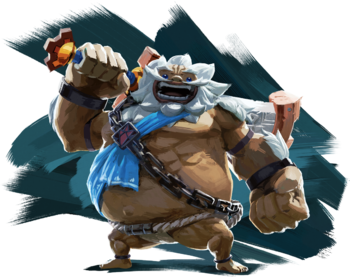
\includegraphics[width=100mm,scale=0.5]{img/daruk.png} \\

eating rocks makes their cultures particularly dependent on mining to survive, to the extent that the majority of gorons have experience in this profession. Many anthropologists believe gorons evolved to be as physically powerful and enduring as they are due to their race's inherent dependency on mining. Stronger gorons with greater strength made better miners, which enabled them to better survive and provide for their kin.\\
Due to their mining dependency, goron culture heavily involves stonework and the working of metals. Blacksmiths are abundant among them, and their structures are constructed almost entirely of metal. They're also one of few races that has widely adapted the use of blackpowder, and when in battle they often make use of bombs or other explosives. Their resistance to heat gives them an edge over most foes when using such powerful, but esoteric weapons.\\
Gorons almost always place a high degree of value on physical strength and stamina, pride, honesty, and trustworthiness. Gorons most readily get along with races which share these values, usually including the like of subrosians, rito, and most hylians. A friend is rarely lost on a goron unless that friend is caught in a lie. Unsurprisingly, gorons often have a difficult time with people from less prideful cultures.

\subsection{Goron Names}
Goron names are all considered male. These names more often than not consist of at least one "go" or "da" syllable. Deep vowel sounds such as "ah," "oh," and "oo" are prominent. "R" consonants are also very common, especially in the center of the name. \\
\textbf{Male:} Biggoron, Darbus, Daruk, Darmani, Darunia, Gongoron, Gorko, Gortram, Kabetta, Kagoron, Medigoron, Reagah, Rohan, Tanko, Volcon, Yunobo. 

\subsection{Goron Traits}
Built like mountains, eating rocks, and wading through lava — gorons are nothing if not hardy and impregnable.
\indent \textbf{Ability Score Increase.} Your Strength score increases by 2 and your Constitution scores increases by 1.\\
\indent \textbf{Age.} Gorons reach adulthood in about a decade, but can live to be over a century. \\
\indent \textbf{Alignment.} Although gorons can alienate those outside their kin group, they form strong bonds with those they trust. They have a tendency towards lawful good.\\
\indent \textbf{Size.} Gorons are usually between 6 and 8 feet in height, and quite stocky. Your size is Medium.\\
\indent \textbf{Speed.} Your base walking speed is 25 feet.\\
\indent \textbf{Hot Skin.} You have resistance to fire damage, and are unable to catch flame.\\
\indent \textbf{Stone Armor.} Your skin is hard as stone. When you aren’t wearing armor and not wielding a shield, your AC is 13 + your Constitution modifier.\\
\indent \textbf{Darkvision.} Accustomed to life underground, you have superior vision in dark and dim conditions. You can see in dim light within 60 feet of you as if it were bright light, and in darkness as if it were dim light. You can’t discern color in darkness, only shades of gray.\\
\indent \textbf{Natural Athlete.} You are proficient in the Athletics skill.\\
\indent \textbf{Like Stone.} You can attempt to hide when you are surrounded by any kind of rocky terrain. Additionally, you can move across difficult terrain made of earth or stone without expending extra movement.\\
\indent \textbf{Stone in the Water.} You sink to the bottom of any body of water you enter. Also, you have no need to drink water, and can hold your breath indefinitely. While underwater, you have disadvantage on all ability checks and attack rolls.\\
\indent \textbf{Goron Roll.} When you take the Dash action, you gain the extra movement you otherwise would plus 20. If you take the Dash action and move at least 20 feet straight towards a creature, you can make a roll attack against that creature as a bonus action. This attack counts as an unarmed strike against the target and its damage is decided by a d4 dice roll plus your Strength modifier. This dice changes as you level up, as shown in the Roll Attack table.
\begin{dndtable}
 	\textbf{Goron Level}  & \textbf{Roll Attack Damage} \\
    1st  & 1d4 + Strength Modifier \\
 	5th  & 1d6 + Strength Modifier\\
  	11th  & 1d8 + Strength Modifier\\
    17th  & 1d10 + Strength Modifier\\
\end{dndtable}
\indent \textbf{Rock Gourmet.} You are able to eat half a pound of rock instead of consuming a portion of rations whenever you feel hungry.\\
\indent \textbf{Languages.} You can speak, read, and write Common and Goro.

% Zora race
\newpage
\section{Zora}

\subsection{Physiology}

Amphibious, fish-like humanoids, zora have sleek and glistening bodies. Zora rarely breed, but when they do, they have offspring in batches of eggs ranging from 1 to 8, which grow into tadpoles, and eventually amphibious humanoids. Zora age at a slow rate compared to hylians, but have a growth spurt and reach adulthood around the age of 20, reach middle age at about 100 years, and can occasionally live to be more than 200.
The exact shape and demeanor of zora is heavily dependent on the two subraces: sea zora, and river zora. "Sea zora" have evolved to live in deeper saltwater, and "river zora" have evolved to live in shallower freshwater, but modern zora of either variety can be found in either habitat.\\
Sea zora are taller and more slender, and have a pale white chest and face, with a backside of a darker color—usually blue, but occasionally red, gray, brown, or other colors. The shape of a sea zora's head varies widely, but usually has a backside resembling some variety of fish tail, with fins that further aid its ability to swim.\\

\subsection{Society}

Due to their amphibious nature, zora villages are most often built along coastlines, rivers, lakes, and other areas that blend shallow water with nearby land. This enables them to effectively evade and defend against predators that are exclusive to land or sea, and hunt more effectively from both sources. Zora usually wear a small amount of jewelry or armor, but less clothing than races such as hylians or rito, as excess clothing hampers their ability to swim.\\
A given zora tribe is usually ruled by a royal family of zora, to which the tribe is loyal for generations. The current monarch of a tribe is often referred to with a title such as "King Zora" or "Queen Zora" than his or her actual name.\\
Royal families are usually allies with the royal families of hylians. They frequently intermingle with other races who live on coastlines, and are renowned for their unique style of music.

\subsection{Zora Names}
Zora names tend to be exotic and easy to pronounce. They are also rarely composed of more than three syllables. \\
\textbf{Male:} Cleff, Japas, Mikau, Ralis, Sidon, Tijo, Toto \\
\textbf{Female:} Laruto, Lulu, Mipha, Oren, Rutela, Ruto 
\newpage
\begin{center}
	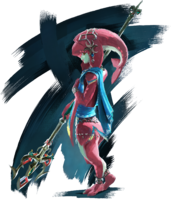
\includegraphics[width=75mm,scale=0.5]{img/mipha.png} \\
\end{center}
\subsection{Zora Traits}
Zora claim the title of the only truly amphibious race in Hyrule — and are the second most populous, exceeded only by hylians.\\
\indent \textbf{Ability Score Increase.} Your Wisdom score increases by 2 and your Dexterity score increases by 1.\\
\indent \textbf{Age.} Zora reach adulthood by the age of 20 at the earliest, and can live to an age of 200 or more.\\
\indent \textbf{Alignment.} Zora tend towards lawful neutral.\\
\indent \textbf{Size.} A zora can vary greatly in size, but is usually about 6 feet tall. Rarely, a zora can grow to a height of 8 feet or more. Your size is Medium.\\
\indent \textbf{Speed.} Your base walking speed is 30 feet, and you have a swim speed of 60 feet.\\
\indent \textbf{Amphibious.} You can breathe both air and water.\\
\indent \textbf{Underwater Camouflage.} When you make a Dexterity (Stealth) check while mostly or entirely underwater, you do so with advantage. \\
\indent \textbf{One with the Water.} You have advantage on all Acrobatics, Animal Handling, Nature and Survival ability checks that involve water or any animal that lives in a wet environment.\\
\indent \textbf{Fire Vulnerability.} You are vulnerable to fire damage attacks.\\
\indent \textbf{Keen Senses.} You have proficiency in the Perception skill.\\
\indent \textbf{Lightning Field.} You can cast the \textit{lightning field} cantrip. Wisdom is your casting ability for this spell. \\
\indent \textbf{Ancestral Arms.} You have proficiency with the pike, net, spear, and trident.\\
\indent \textbf{Languages.} You can speak, write, and read Common and Zoran.
\newpage
% Korok race

\section{Korok}

\subsection{History}

According to legend, koroks were originally created many eons ago by the Great Deku Tree to spread plant life across the entire world. This legend portends that every tree which still grows can trace its ancestry back to a seed planted by a korok. Regardless of whether or not this is true, modern koroks are clearly magical creatures not directly related to any other races, and they retain an unusually profound understanding of the natural world.\\
Despite the innate curiosity of koroks, they are dissuaded by the Deku Tree from leaving the forest unless they have an important reason to do so. Indeed, the world outside the woods is dangerous to a typical korok. In the modern world, few people who dwell outside of forests know much of this race. They are so rare, so bizarre, and so elusive that they are frequently delegated to myth.

\subsection{Physiology}

A typical korok stands between 2 and 3 feet, with an oblong body composed of hollow wood, and particularly short limbs. Indeed, koroks are extremely lightweight and buoyant.\\
A korok's face is most unusual. If left unadorned, a korok face is comprised only of a nose-like stick protruding outward. Almost every korok will instead construct a mask to serve as its apparent face. This mask almost always is comprised of a large leaf with holes cut into it—one hole to anchor the mask on its "nose," two holes to serve as "eyes," and finally one to serve as a "mouth." Koroks seemingly have no physical need to construct these masks, but it is done in part so they can express their personality and in part so koroks can better recognize each other. Koroks tend to be very fascinated by creatures who are naturally more expressive than themselves, and it seems these masks are modeled after such creatures.\\
Although koroks can be created by the Deku Tree's magic, they can also reproduce on their own, unlike kokiri. A korok can produce more koroks simply by planting seeds and caring for them until they grow to maturity, although this is a relatively rare practice performed only a few times in a korok's long lifespan. Despite technically being parent and child, these two koroks would consider themselves more akin to an older sibling and a younger one.\\
A korok reaches its full size less than two years after being planted, and usually gains mobility a long time before that. The earliest a korok can produce a seed of its own seems to be about 2 or 3 years, but it will often live for decades before it decides to do so.\\
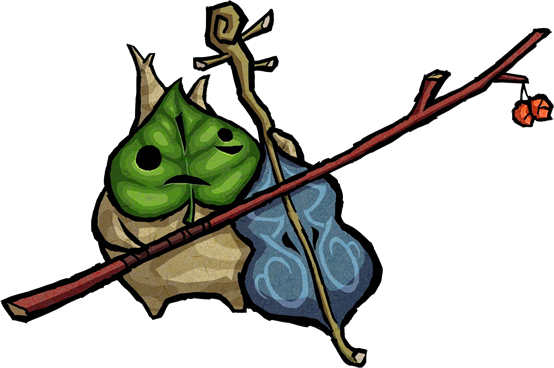
\includegraphics[width=100mm,scale=0.5]{img/makar.png} \\
As they don't reproduce sexually, koroks don't have traditional genders. They don't truly consider themselves male, unlike the all-male goron race, but usually default to male pronouns anyway.

\subsection{Society}

Koroks tend to be very optimistic, curious, altruistic, excitable, energetic, and playful.\\
They predominantly live in forests protected by the Great Deku Tree, often among kokiri, and usually only leave these woodlands temporarily. Much like kokiri, they are considered the "children" of the Deku Tree. They are much more widespread than kokiri, however, likely due to the fact they can reproduce on their own.\\
A korok's needs and therefore its responsibilities are simple. It doesn't require food, can fly or hide from most herbivores, can sleep almost anywhere, and doesn't need to care for its young nor bother much with reproduction. A korok is nonetheless restless and eager to do something—anything. Thus, a typical korok often occupies much of its time playing elaborate games, or exploring the vast wilderness of Hyrule. Many pursue a self-learned art, profession, or expertise—something it can master over the many years it lives. When the Deku Tree has a job that needs doing, there's always at least one korok eager to do it.\\
Perhaps because of this energetic nature, the surprisingly few times koroks interact with races outside the forest, they are nothing but helpful. Many a legend has been told of these altruistic but secretive creatures—completing chores will hylians sleep, saving children from wells, and so on.\\

\subsection{Korok Names}

Korok names tend to be rather short, rarely comprised of more than two brief syllables.\\
\textbf{Examples:} Aldo, Chio, Daz, Drona, Elma, Hestu, Hollo, Irch, Kula, Linder, Maca, Makar, Oakin, Olivio, Pepp, Peeks, Natie, Rown, Walton 

\subsection{Korok Traits}

Small, peaceful, immortal, and child-like plant creatures. They aren't much for combat or stealth, but it's hard not to smile around them.\\
\indent \textbf{Ability Score Increase.} Both your Charisma and Dexterity scores increase by 2. On the other hand, your Constitution score decreases by 1.\\
\indent \textbf{Age.} A korok reaches physical maturity after less than 2 years, but can live for up to 200 years or more. It retains a childlike innocence throughout its entire life.\\
\indent \textbf{Alignment.} Koroks strive to populate the world with trees, preserve life, and are eagerly help anyone who needs it. They have an extreme tendency towards all forms of good.\\
\indent \textbf{Size.} A typical korok’s height averages about 3 feet. Your size is Small.\\
\indent \textbf{Speed.} Your base walking speed is 25 feet.\\
\indent \textbf{Type.} You are considered both a humanoid and a plant for any effect relating to your type.\\
\indent \textbf{Natural Cantrip.} You know the druidcraft cantrip.\\
\indent \textbf{Jingle.} Your body produces an unusual jingling noise whenever you move, which grows louder the more violently you move. You have disadvantage on Dexterity (Stealth) checks to move quietly.\\
\indent \textbf{Fire Vulnerability.} You are vulnerable to all sorts of fire damage. \\
\indent \textbf{Korok Copter.} As an action, you can grow from your wrist a magical plant that is as tall as your body, and adorned with a pair of spinning wings. You can control the wings of this plant in such a way that you effectively gain a flying speed of 25 feet. Maintaining flight requires dedication from this hand, preventing that hand from being used for anything else, but otherwise maintaining flight or hovering in place is effortless for you. You can detach the magical plant as an action or bonus action, which causes it to wither away into ash almost instantly. Until you dismiss the plant, it is considered part of your body, and any damage dealt to it is dealt to you.\\
\indent \textbf{Natural Performer.} You are proficient in both the Performance and the Nature skills. Additionally, you can survive without food, so long as you have water, sunlight, and air.\\
\indent \textbf{Ancient Knowledge.} You gain proficiency in one of the following skills: Arcana, History, Medicine or Religion. Alternatively, you can gain proficiency in any one tool.\\
\indent \textbf{Tool Proficiency.} Most koroks adapt to a particular profession. You gain proficiency in one artisan's tool or one musical instrument of your choice.\\
\indent \textbf{Nature's Guise.} You can attempt to hide when surrounded by any area that is filled with trees or even when you are only lightly obscured by foliage, heavy rain, falling snow, mist, and other natural phenomena.\\
\indent \textbf{Languages.} You can speak, write and read both Common and Deku.

\newpage
% Rito race
\section{Rito}

\subsection{Physiology}
Avian humanoids covered in feathers, rito are particularly tall and thin compared to hylians. Their narrow bodies and hollow bones make them very lightweight for their height and arm span, which eases flight. Indeed, rito have arms that double as wings, and are able to fly as a bird does. Coastal rito have hylian-like arms that slide into "sleeves" they use as wings, whereas highland rito simply have functional hands on the tips of their wings.\\
Rito form families and raise their hatched young one at a time over many years, in a manner very similar to hylians. A rito usually doesn't gain flight until an age of about 10 years, although the means of gaining flight varies between different rito tribes. An adult rito that is unable to fly, a fokka, is usually banished from its tribe and alienated by most rito.

\subsection{Society}
Due to their ability to fly, rito villages are built on mountains, islands, or other locations where most predators have difficulty reaching. Such villages are usually situated near oceans, rivers, or other fish-filled reservoirs. Although rito are omnivorous, their tribes survive primarily from hunting and fishing, and usually only partake in farmed food when it is produced by other races.\\
Rito culture places a relatively high value on honor and order. Postmen in Hyrule are almost universally rito, and their villages rapidly and efficiently sort parcels for all the land.

\subsection{Rito Names}
A rito's name often ends in "-li," and is frequently comprised of three syllables.\\
\textbf{Male:} Gesane, Harth, Huck, Illari, Kaneli, Kass, Kogoli, Koboli, Komali, Mazli, Nekk, Quill, Revali, Verla\\
\textbf{Female:} Amali, Bedoli, Cecili, Lalssa, Medli, Misa, Molli, Namali, Saki

\subsection{Rito Traits}
Rito are a versatile race, able to winged flight and masters of aerial combat.\\
\indent \textbf{Ability Score Increase.} Your Dexterity score increases by 2 and your Wisdom score increases by 1.\\
\indent \textbf{Age.} A rito reaches adulthood in its late teens, and rarely lives to see a century.\\
\indent \textbf{Alignment.} Rito are inherently dutiful, loyal, and stick to their convictions. They tend towards law. \\
\indent \textbf{Size.} An adult rito has a height of about 5 to 7 feet. Your size is Medium.

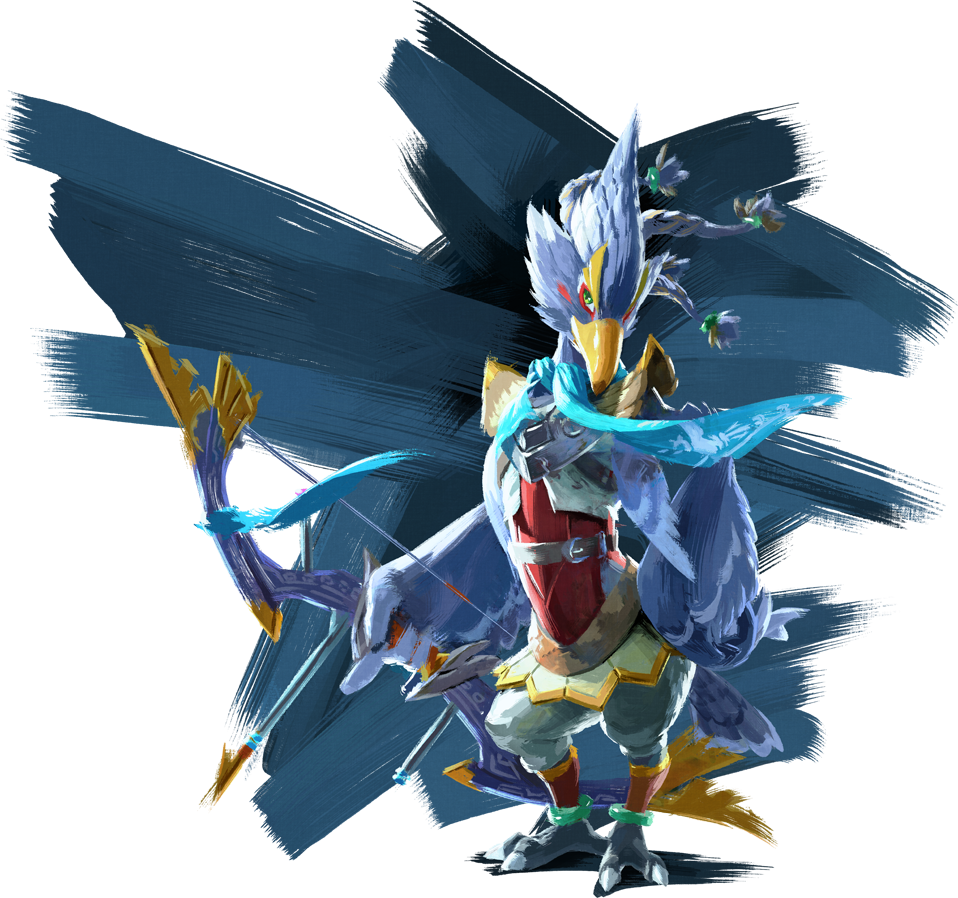
\includegraphics[width=100mm,scale=0.5]{img/revali.png} \\

\indent \textbf{Speed.} You have a base walking speed of 25 feet.\\
\indent \textbf{Flight.} You have a flying speed of 50 feet. To use this
speed, you can’t be wearing medium or heavy armor.
\indent \textbf{Aerial Combat.} You have proficiency with the shortbow and the longbow. Additionally, you have advantage on Acrobatic skill checks while flying.\\
\indent \textbf{Languages.} You can speak, read, and write Common and one extra language of your choice. Rito typically learn the languages of other peoples they deal with, including obscure dialects.

\newpage
% Deku race
\section{Deku}
\subsection{Physiology}
An adult deku scrub stands at a height ranging between roughly 2 and 4 feet, and weighs somewhere between 25 and 50 pounds. Scrubs have skin comprised of tree-like bark, and they feature outgrowths of leaves used to absorb sunlight and perform a process similar to photosynthesis. Nearly all deku scrubs have some form of leaves or shrubbery growing from atop their heads, though many of them style it in ways other than the typical wild look. Most also grow leaves below their neck and across their torsos, which other races might mistake for clothing. Though rare, deku scrubs can also grow flower petals alongside or in place of leaves—and this is usually considered a feminine quality.\\
Deku scrubs have yellow, orange, or red eyes which glow dimly and allows many of them to see in darkness. Rather than a nose or a mouth, their face features a short tubular 'snout' which can both smell and taste that which enters it. Most deku scrubs are able to move their snout from its default circular shape, especially with practice—and those who live among other races often to so to more easily convey emotions to races prone to smiling and frowning. These snouts are frequently used to spit nuts at high speed, used as both a means of warding off predators and as a means of reproduction.\\

\subsection{Gender and Life Cycle}
Like most plants, deku scrubs are effectively hermaphrodites, as there are no physiological differences to differentiate gender. Scrubs who are influenced by gendered races usually adapt a gender for themselves, but this usually depends only on whether the deku scrub feels like a more masculine or feminine individual. Male is chosen more often than not.\\
To a deku scrub, the seeds its body produces are more of a means of weaponry than of reproduction. Creating a seed requires very little resources on behalf of the scrub, but it is draining enough that a deku scrub usually only does so when it feels threatened. When a scrub does spit one of its seeds, that seed rarely finds soil and nutrients enough to grow. When it does, the seed gradually grows into a deku scrub in its own right, usually with no dependency on parents. Indeed, the concept of a special parent-child relationship is foreign to all but the most cultured of deku scrub tribes.\\
After conception, a deku scrub is effectively immobile, dependent on the environment—or friendly caregivers—to receive sunlight, water, and other nutrients. During this period, lasting a few years, the immobile deku scrub may be affected by the pollen of other deku scrubs in the area, and consequently be influenced by their genes. Once the period ends, the deku scrub grows legs, and its mobile body is able to separate from a rooted part of the plant—a "deku flower"—that is left behind where the scrub was planted. By this point, the deku scrub gains something resembling sentience. Curiously, deku scrubs at this stage inherently know some basic words and phrases in the Deku language. Indeed, it is believed the entire Deku language is based on the basic words all scrubs seem to know.\\
The body of a young deku scrub only has legs, an abdomen, and a head. It doesn't gain arms until it reaches a certain age—wildly varying from 5 to 15. Some never grow any arms at all, though this is usually an inherited deficiency.\\
Deku scrubs are most at home while nesting in their deku flowers, as the flowers are both physically comfortable provide additional nutrients that are otherwise difficult to obtain. Many a scrub spends its entire life comfortably resting inside its own flower. Some scrubs instead move from one flower to the next, renting and trading prime locations in the same way other races trade in real estate. A deku scrub can generally gain the same nutritional and nesting benefits from any deku flower. Although it is unpleasant, a rare few deku scrubs give up reliance on deku flowers entirely for the sake of independence.

\subsection{Society}
Due to their means of reproduction, many deku scrubs don't think of themselves as part of a "society," and are inherently very individualistic. They usually only find family in other deku scrubs that were planted near them by happenstance, and have no traditional roles such as parent, child, or sibling. They are inherently distrustful of any creatures not of this family, even other deku scrubs. Such scrubs instinctively spit nuts at strangers to ward them off—a habit many deku scrubs have difficulty breaking.\\
Although this simple life is tradition, in the past few centuries some deku scrubs have learned to organize and culture themselves more like other races. A few families have even formed their own small kingdoms in swamps, forests, or other places of abundant flora. These kingdoms have adapted many cultural habits from other races, most notably hylians, such as building wooden structures or forming small but organized armies.\\
There are a few rare scrubs who intermingle with hylians, gorons, and other more hospitable races. These deku scrubs tend to fancy themselves as businessmen and traders, or occasionally adventurers. Even these civilized scrubs have a tendency towards erratic behavior, paranoia, and other unusual habits compared to the likes of hylians.

\subsection{Deku Names}
Names are less important to deku scrubs than to most other races. They are often born without a name, and usually only give themselves a name when interacting with hylians or other races with which names are important. Even then, it is usually some variation on "Deku," such as Dekki or Deppi.\\
Within the most organized of deku scrub societies different scrubs are usually referred to by their occupation or another title, such as "Deku King" or "Deku Butler." As their tribes are isolated and rarely exceed a hundred, this remains effective for them.

\subsection{Deku Traits}
Small, wooden, and sharing many characteristics with plants — most other races find deku scrubs a bit odd.\\
\indent \textbf{Ability Score Increase.} Your Dexterity score increases by 2.\\
\indent \textbf{Age.} Deku scrubs do not become mobile for 2 or 3 years after being planted, and do not reach adulthood until the mid teens. Most can live to an age of 70.\\
\indent \textbf{Alignment.} Deku scrubs are often paranoid, irrational, and tend to live selfishly. They tend towards chaos. \\
\indent \textbf{Size.} Deku scrubs range in height from 2 to 4 feet. Your size is Small.\\
\indent \textbf{Speed.} Your base walking speed is 25 feet.\\
\indent \textbf{Type.} You are considered both a humanoid and a plant for any effect relating to your type.\\
\indent \textbf{Darkvision.} You can see in dim light within 60 feet of you as if it were bright light, and in darkness as if it were dim light. You can't discern color in darkness, only shades of gray.\\
\indent \textbf{Seed Shot.} Your funnel-like snout can Deku Nuts that are naturally produced by your body, and you can shoot a seed as a ranged weapon attack without using your hands. If you hit with it, you deal bludgeoning damage equal to 1d4 + your Dexterity modifier. This attack has a range increment of 20/60 ft. You are proficient with this weapon.\\
\indent \textbf{Fire vulnerability.} Due to your body being made of wood, you are vulnerable to fire damage.\\
\indent \textbf{Water Hop.} Dekus are unable to swim. However, when you use the Dash action while your speed is not reduced, you can traverse over the surface of water or similar liquids until the end of your turn. If your turn ends while you are over a liquid, you will submerge to the bottom. Additionally, Dekus are also able to stand on floating plants such as lily pads and can last twice as long underwater when compared to other races.\\
\indent \textbf{Naturalist.} You have proficiency in the Nature skill.\\
\indent \textbf{Forest Camouflage.} You have advantage on Dexterity (Stealth) checks made to hide in forests, woodlands, or other terrain of abundant foliage.\\

\begin{center}
    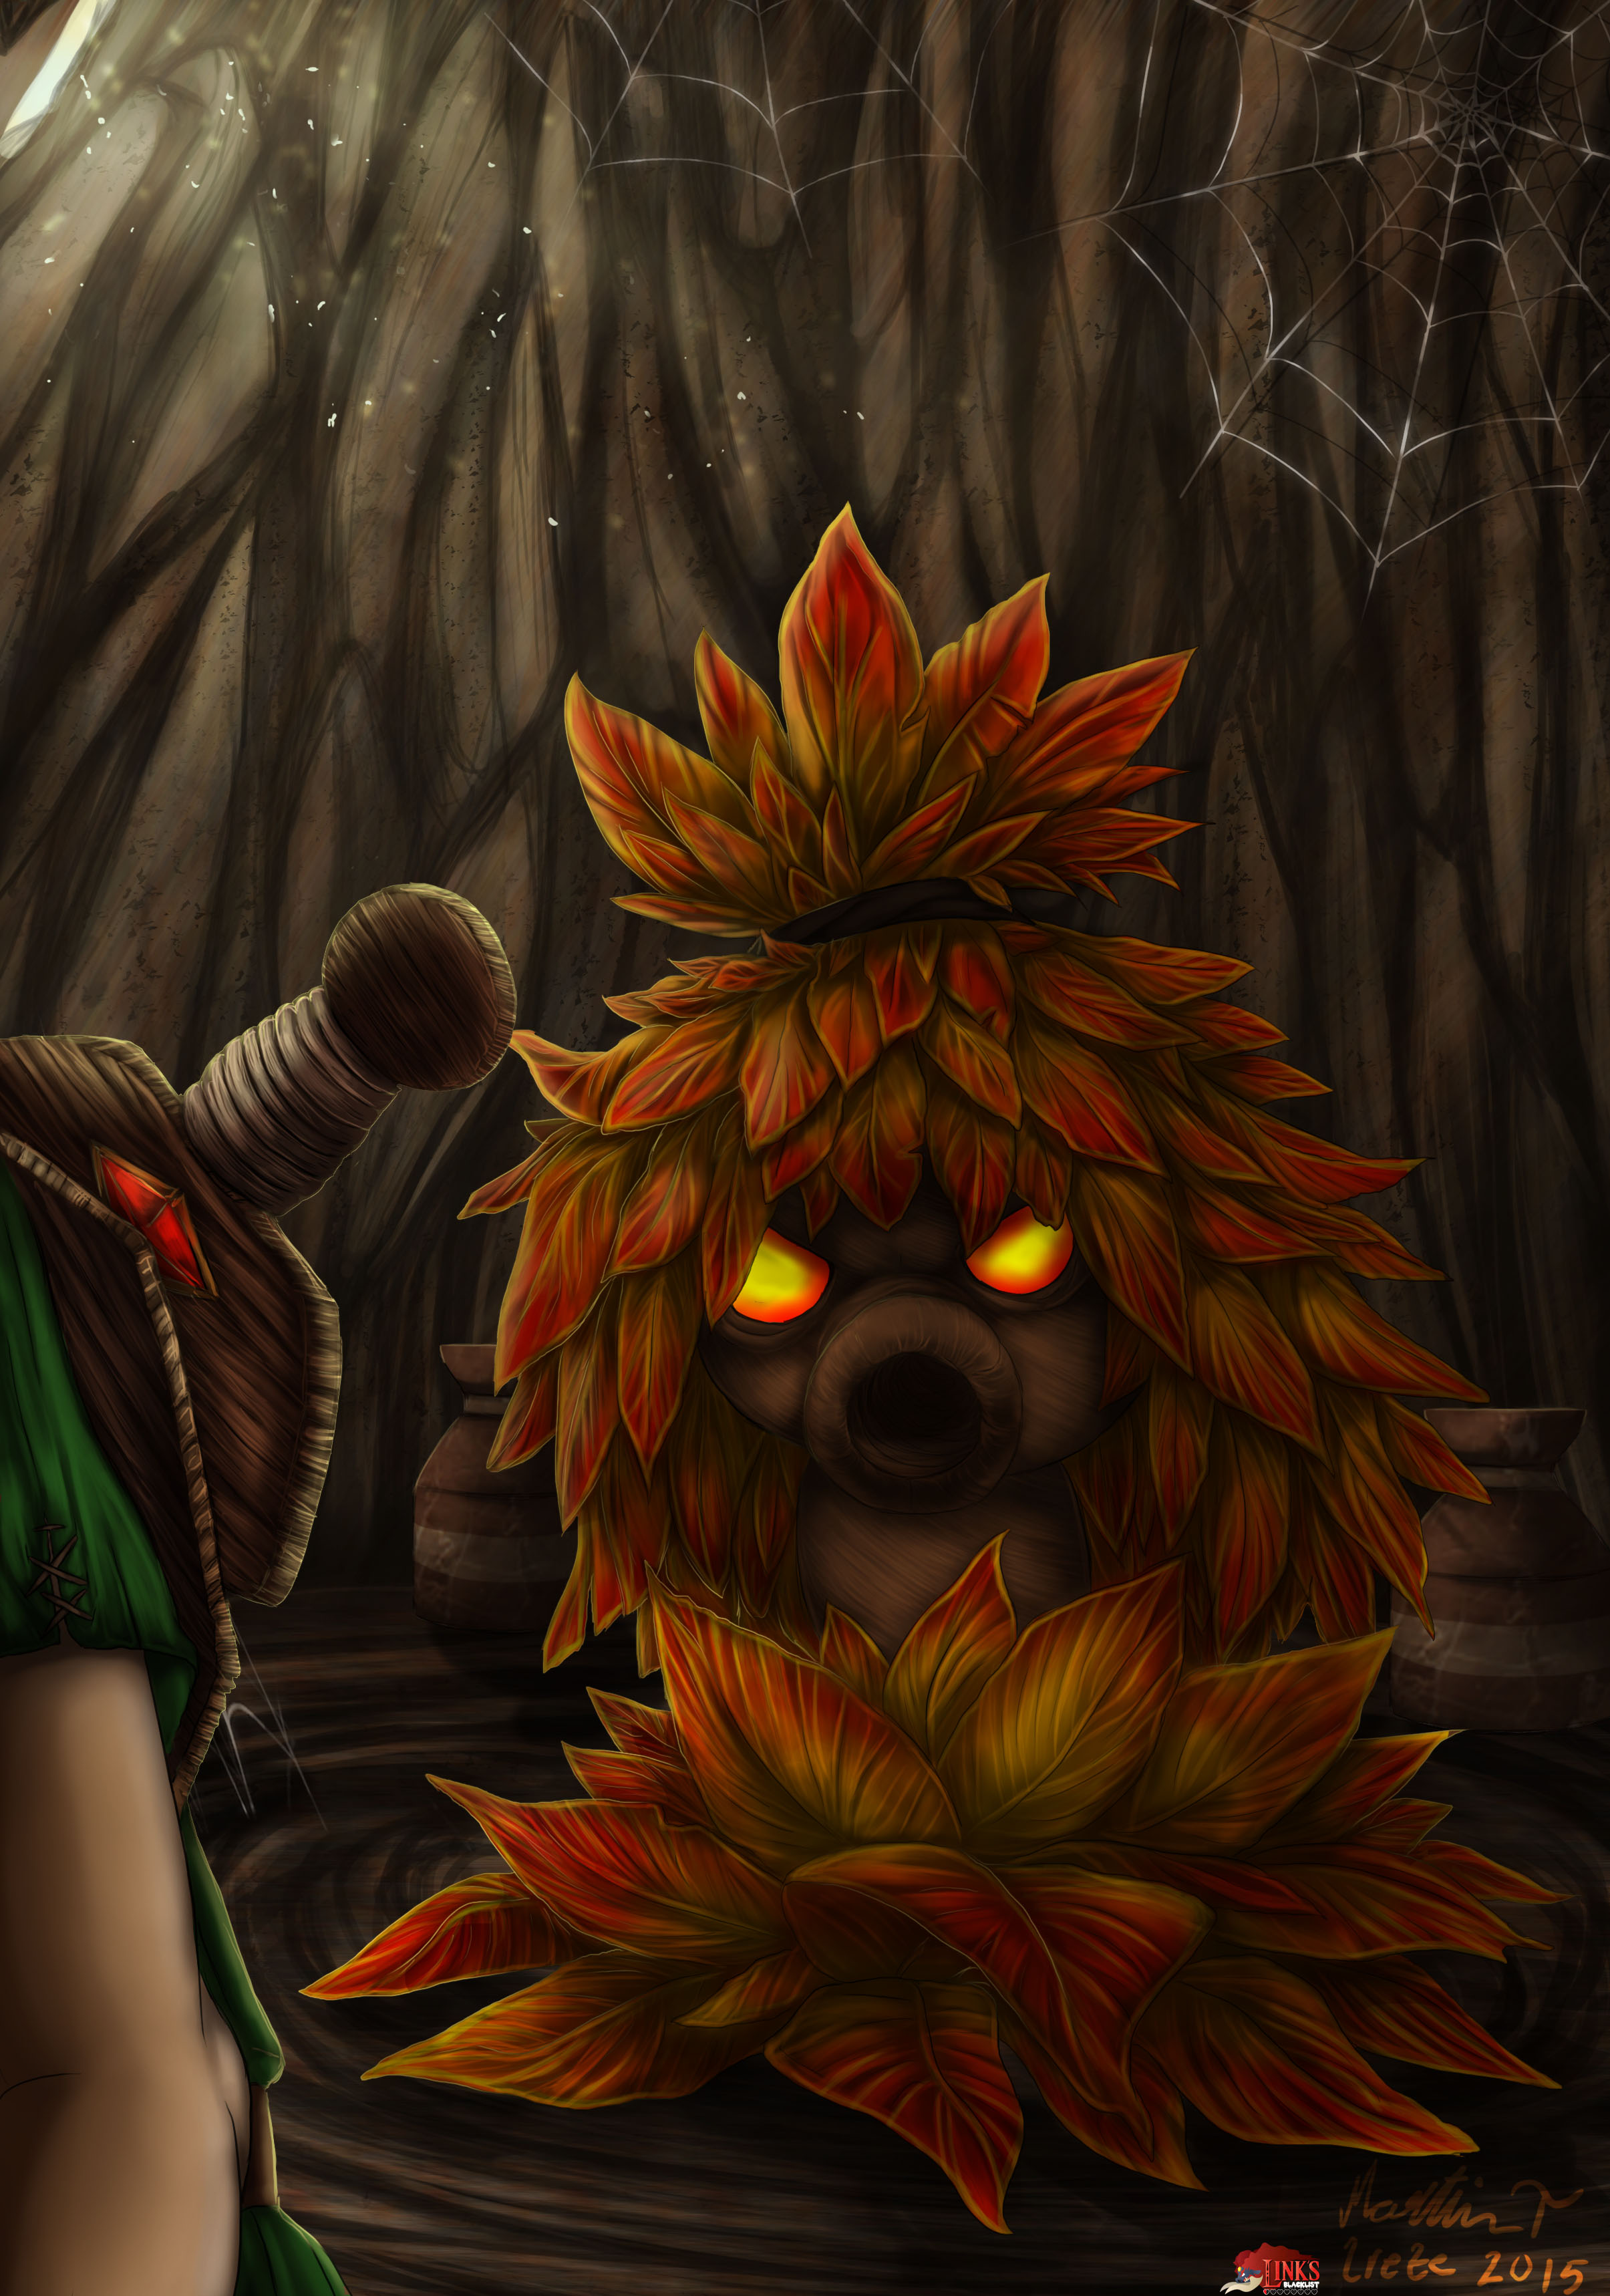
\includegraphics[width=70mm,scale=0.5]{img/deku.jpg} 
\end{center}

\indent \textbf{Deku Flight.} Deku are able to use Deku Flowers to launch themselves to normally unreachable places by casting the \textit{petal glide} cantrip.\\
\indent \textbf{Languages.} You can read, write, and speak Common and Deku.\\
\indent \textbf{Subraces.} Two major subraces of deku are found among the worlds of Hyrule and Termina: swamp deku and forest deku. Choose one of these subraces.

\subsubsection{Swamp Deku}
As a swamp deku, you have increased resilience and have adapted to the environment you live in. Swamp deku recognize that there is order and they belong to kingdoms controlled by the deku royal family.\\
\indent \textbf{Ability Score Increase.} Your Constitution score increases by 1.\\
\indent \textbf{Poison Resistance.} You have advantage on saving throws against poison, and you have resistance to poison damage.

\subsubsection{Forest Deku}
Forest deku are more disorganized when compared to swamp deku and tend to remain in the forest they were born in. They are protectors of the forest they were born in, and are able to easily find themselves in mazes, forest, and groves.\\
\indent \textbf{Ability Score Increase.} Your Wisdom score increases by 1.\\
\indent \textbf{Forest Pathfinder.} Your base movement speed increases by 5 feet. Additionally, you have advantage on Nature skill checks made in a forest environment.

% Backgrounds
\chapter{Backgrounds}

\subsection{Village Champion}
You always possessed the heart of a hero. Need a dragon to be slain? Is a wolf slaughtering a local farmer's sheep? Has the village elder's daughter been recently abducted? Whatever it is, you are the one for this job.\\
Some do it for the glory, others do it to get payed, and some do it, because they are just altruistic. Whatever the reason is, they know how to call.\\

\noindent \textbf{Skill Proficiencies:} Intimidation, Survival\\
\textbf{Tool Proficiencies:} One type of gaming set\\
\textbf{Languages:} Your journeys have taken you far. Learn a standard language of your choice that was used during your travels.\\
\textbf{Equipment:} A gaming set (one of your choice), a shovel, an iron pot, a set of common clothes, a trinket that is involved on the quest to save your village, and a belt pouch containing 10 gp.

\subsubsection{Defining Event}
Doesn't matter what you were in your "past life", you are a hero now. But every champion has to start somewhere. Choose or randomly determined the first event that marked your life as a champion.

\begin{dndtable}
 	\textbf{d6}  & \textbf{Defining Event} \\
    1  & I stood up to a tyrant’s agents. \\
 	2  & I saved people during a natural disaster.\\
  	3  & I stood alone against a terrible monster.\\
    4  & Recruited into a lord’s army, I rose to leadership and was commended for my heroism.\\
    5  & I found the artifact that saved my people from imminent disaster.\\
    6  & I bested the village's champion before me, taking the mantle.\\
\end{dndtable}

\subsubsection{Feature: Presence of a Hero}
Renown for your strength, valor and resolution, townsfolk who have heard of your deeds will look for you to help them with troubles they are currently facing. Additionally, these honest vendors and villagers who are seeking your good graces will might offer you small discounts for a variety of good and services. 

\subsubsection{Suggested Characteristics}
A champion is the hero of his village, city, town or region, for better or for worse. Most common folk and nobles rely on the champion to secure their lives and the future of their origin.

\begin{dndtable}
 	\textbf{d8}  & \textbf{Personality Trait} \\
    1 & I judge people by their actions, not their words. \\
    2 & If someone is in trouble, I’m always ready to lend help. \\
    3 & I get bored easily. When am I going to get on with my
destiny? \\
    4 & I’m confident in my own abilities and do what I can to
instill confidence in others. \\
    5 & When I set my mind to something, I follow through no
matter what gets in my way. \\
    6 & Thinking is for other people. I prefer action. \\
    7 & There is always the need for an action plan. \\
    8 & There is no plan B or C. I only planned A. \\
\end{dndtable}

\begin{dndtable}
 	\textbf{d6}  & \textbf{Ideal} \\
	1 & \textbf{Respect.} People deserve to be treated with dignity and respect (Good) \\
    2 & \textbf{Fairness.} No one should get preferential treatment before the law, and no one is above the law. (Lawful) \\
    3 &  \textbf{Freedom.} Tyrants must not be allowed to oppress the people. (Chaotic) \\
    4 &  \textbf{Might.} If I become strong, I can take what I want—what I deserve. (Evil) \\
    5 &  \textbf{Reflection.} Every deed has its price.(Neutral) \\
    6 &  \textbf{Destiny.} Nothing and no one can steer me away from my higher calling. (Any) \\
\end{dndtable}
\newpage
\begin{dndtable}
 	\textbf{d6}  & \textbf{Bond} \\
     1  & I made a promise to keep the village safe long ago. I intend to keep it.\\
     2  & I hold the knowledge to save my people from incoming danger. Only I can help them.\\
     3  & Destruction is at hand, and, even though I am not one of the best, I am the only warrior our village has left.     \\
     4  & I am considered to be the best fighter in my village; therefore, I am the one who should protect it.\\
     5  & Nothing is capable of standing between me and my friends.\\
     6  & I love my village, and I'll do anything to protect it.\\
\end{dndtable}

\begin{dndtable}
 	\textbf{d6}  & \textbf{Flaw} \\
	1  & If there’s a plan, I’ll forget it. If I don’t forget it, I’ll
ignore it.\\
	2  & I’m convinced of the significance of my destiny, and
blind to my shortcomings and the risk of failure.\\
	3  & I have trouble trusting in my allies.\\
	4  & I have a weakness for the vices of the city, especially
hard drink.\\
	5  & I’ll do anything to win fame and renown.\\
	6  & I’m a sucker for a pretty face.\\
\end{dndtable}
\\

\subsection{Royal Family Member}
You are part of your race's royal family. Tradition, wealth, land, and power are matters that you can't cast aside. You had access to the best education, the best health care, and you learned important lessons from your family members. Moreover, you are well aware that your actions represent your family as a whole, and therefore, must be willing to keep that reputation at the highest rating possible. And while there is matters that you can use your resources to do the work for you, sometimes you must get personal. After all, if you want a job well done, you must do it yourself.\\

\noindent \textbf{Skill Proficiencies:} History, Persuasion\\
\textbf{Tool Proficiencies:} One type of gaming set\\
\textbf{Languages:} One of your choice\\
\textbf{Equipment:} A set of fine clothes, a scroll of pedigree, a valuable trinket, and a purse containing 30 gp.

\subsubsection{Feature: High Society}
Being part of the royal family means you are able to participate in all social events that involve high society without having an invitation. This does not involve secret or common folk events. Additionally, you have ease in securing an audience with a local member of a high family and have a personal messenger to receive and send messages to your family so as to know the necessities and welfare of your kingdom and your family.


\subsubsection{Suggested Characteristics}
High birth means you are raised to a very different lifestyle than most people ever experience, and your personality reflects that upbringing. Being a member of the royal family means you have responsibilities and bonds not only to your family, to your lands, but to the people that serve you. However, that doesn't mean you can't serve yourself. 


\begin{dndtable}
 	\textbf{d8}  & \textbf{Personality Trait} \\
    1 & My eloquent flattery makes everyone I talk to feel
like the most wonderful and important person in the
world. \\
    2 & The common folk love me for my kindness and
generosity. \\
    3 & I take great pains to always look my best and follow the
latest fashions. \\
    4 & I don’t like to get my hands dirty, and I won’t be caught
dead in unsuitable accommodations. \\
    5 & Despite my noble birth, I do not place myself above
other folk. We all have the same blood. \\
    6 & I am not responsible if you are miserable. We all draw our own paths. \\
    7 & My favor, once lost, is lost forever. \\
    8 & I am beyond the common folk and nobles. I deserve so much more. 
\end{dndtable}
\newpage

\begin{dndtable}
 	\textbf{d6}  & \textbf{Ideal} \\
	1 & \textbf{Respect.} Respect is due to me because of my position,
but all people regardless of station deserve to be treated with dignity. (Good) \\
    2 & \textbf{Independence} I must prove that I can handle myself without the coddling of my family. (Chaotic) \\
    3 &  \textbf{Family.} Blood runs thicker than water. (Any) \\
    4 &  \textbf{Obligation.} It is my duty to protect and care for
the people beneath me. (Good) \\
    5 &  \textbf{Power.} If I can attain even more power, I will increase my family's control. (Neutral)\\
    6 &  \textbf{Ascension} I must claim the throne of power, even if it is not my birthright. Whatever. It. Takes. (Evil) \\
\end{dndtable}

\begin{dndtable}
 	\textbf{d6}  & \textbf{Bond} \\
     1  & I will face any challenge to win the approval of my family.\\
     2  & Nothing is more important than the other members of my family.\\
     3  & I am in love with the heir of a family that my family despises.\\
     4  & The common folk must see me as a hero of the people.\\
     5  & Nothing is more important than remaining in power.\\
     6  & My family's alliance with another kingdom must be sustained at all costs.\\
\end{dndtable}

\newpage
\begin{dndtable}
 	\textbf{d6}  & \textbf{Flaw} \\
	1  & I secretly believe that everyone is beneath me.\\
	2  & I hide a truly scandalous secret that could ruin my family forever.\\
	3  & I too often hear veiled insults and threats in every word addressed to me, and I’m quick to anger.\\
	4  & I have an insatiable desire for carnal pleasures. \\
	5  & In fact, the world does revolve around me.\\
	6  & By my words and actions, I often bring shame to my family.\\
\end{dndtable}
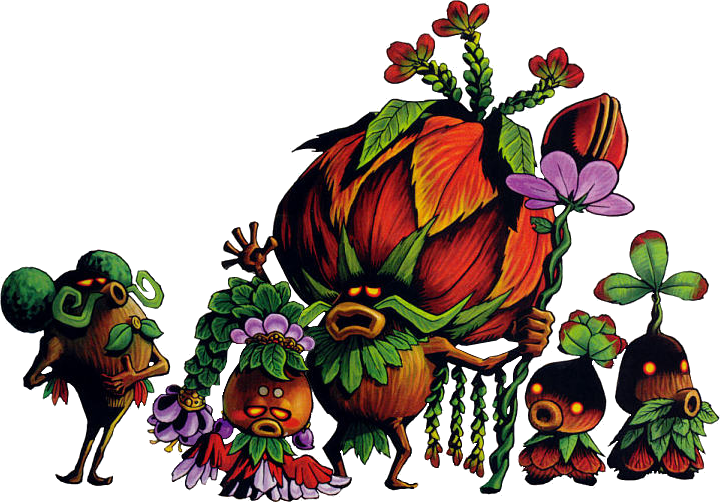
\includegraphics[width=100mm,scale=0.5]{img/deku_royal_family.png} \\
% Spells from the world of Hyrule
\chapter{Hyrule Spells}
%The spells are presented in alphabetical order.

\section{Lightning Field}
\textit{Evocation Cantrip} \\

\noindent \textbf{Casting Time:} 1 action\\
\textbf{Range:} 5 feet\\
\textbf{Components:} S\\
\textbf{Duration:} Instantaneous\\

\noindent A cylindrical aura of electricity sweeps around you for a moment, jolting adjacent foes. Each creature within range, other than you, must succeed on a Dexterity saving throw or take 1d6 lightning damage. \\
This spell's damage increases by 1d6 when you reach 5th level (2d6), 11th level (3d6), and 17th level (4d6). \\

\section{Petal Glide}
\textit{Conjuration Cantrip} \\

\noindent \textbf{Casting Time:} 1 action\\
\textbf{Range:} 5 feet\\
\textbf{Components:} S, M (a flower petal)\\
\textbf{Duration:} Concentration, up to 1 minute\\

\noindent You manifest a large, lightweight, and daisy-like flower as tall as a human. It appears harmlessly in your hand or anywhere within the range of this spell. When the stem of this conjured flower is gripped in the hand, it magically rotates to generate thrust. A Medium or smaller creature who grasps the stem in its hand immediately flies straight upward a distance of 30 feet, and gains a fly speed of 30 feet for so long as it holds the stem. The benefiting creature cannot ascend higher with this fly speed without the aid of an updraft or similar force. If the creature releases the stem or this cantrip's duration ends, the flower vanishes into thin air. This cantrip can only be cast when standing or inside a Deku Flower. \\

%\begin{commentbox}{Neat Green Box!}
%	\lipsum[1]
%\end{commentbox}

%\subtitlesection{Weapon, +1, +2, or +3}
%{Weapon (any), uncommon (+1), rare (+2), or very rare (+3)}

%\begin{quotebox}
%	As you approach this template you get a sense that the blood and tears of many generations went into its making. A warm feeling welcomes you as you type your first words.
%\end{quotebox}

%\newpage % Acts as columbreak because of twocolumn option; for pagebreak use \clearpage

% For more columns, you can say \begin{dndtable}[your options here}.
% For instance, if you wanted three columns, you could say
% \begin{dndtable}{XXX}. The usual host of tabular parameters are
% aailable as well.
%\header{Nice table}


%\begin{paperbox}{Do the Players need direction?}
%	\lipsum[1]
%\end{paperbox}

% You can optionally not include the background by saying
% begin{monsterboxnobg}
\begin{comment}
\begin{monsterbox}{Monster Foo}
	\textit{Small metasyntactic variable (goblinoid), neutral evil}\\
	\hline
	\basics[%
	armorclass = 12,
	hitpoints  = 16 (3d8 + 3),
	speed      = 50 ft
	]
	\hline
	\stats[
    STR = \stat{12}, % This stat command will autocomplete the modifier for you
    DEX = \stat{7}
	]
	\hline
	\details[%
	% If you want to use commas in these sections, enclose the
	% description in braces.
	% I'm so sorry.
	languages = {Common Lisp, Erlang},
	]
	\hline \\[1mm]
	\begin{monsteraction}[Monster-super-powers]
		This Monster has some serious superpowers!
	\end{monsteraction}
	\monstersection{Actions}
	\begin{monsteraction}[Generate text]
		This one can generate tremendous amounts of text! Though only when it wants to.
	\end{monsteraction}

	\begin{monsteraction}[More actions]
    See, here he goes again! Yet more text.
	\end{monsteraction}
\end{monsterbox}
\end{comment}
% End document
\end{document}
